\documentclass[a4paper,oneside,12pt]{book}

%----------------------------------------------------------------------------------------
%	PAPER INFORMATION
%----------------------------------------------------------------------------------------

\newcommand{\thesistitle}{AI-Assisted Ethics Assessment for Early-Stage Research Projects: An Ontology-Driven Knowledge Graph and Retrieval-Augmented Generation Approach}
\newcommand{\degree}{MSc Computer Science (Intelligent Systems)}
\newcommand{\typeofthesis}{research paper}
\newcommand{\authorname}{Navina Ganapathy Amuthan}
\newcommand{\supervisor}{Prof. Dave Lewis}
\newcommand{\keywords}{AI ethics, ontology, knowledge graph, retrieval-augmented generation, EU AI Act, fundamental rights, ethics assessment, REAMS, compliance automation}
\newcommand{\school}{\href{https://www.tcd.ie/scss/}{School of Computer Science and Statistics}}
\newcommand{\college}{Trinity College Dublin}

%% Language and font encodings
\usepackage[T1]{fontenc}
\usepackage[utf8]{inputenc}
\usepackage[english]{babel}

%% Bibliographical stuff
\usepackage[]{cite}
%% Document size
\usepackage[a4paper,top=2.54cm,bottom=2.54cm,left=2.54cm,right=2.54cm,headheight=16pt]{geometry}
\setlength{\marginparwidth}{2cm}
%% Useful packages
\usepackage{amsmath}
\usepackage[autostyle=true]{csquotes}
\usepackage[pdftex]{graphicx}
\usepackage[colorinlistoftodos]{todonotes}
\usepackage[colorlinks=true, allcolors=black]{hyperref}
\usepackage{hyperxmp}
\usepackage{caption}
\usepackage{sfmath}
\usepackage[parfill]{parskip}
\usepackage{setspace}
\usepackage{enumerate}
\usepackage{booktabs}
\usepackage{fancyhdr}
\usepackage{xcolor}
\usepackage{longtable}
\usepackage{multirow}
\usepackage{array}
\usepackage{listings}
\usepackage{url}
\numberwithin{equation}{chapter}
\pagestyle{plain}

\definecolor{tcd_blue}{RGB}{5, 105, 185}

\renewcommand{\familydefault}{\sfdefault}

%% Format Chapter headings
\usepackage{titlesec}
\titleformat{\chapter}[hang]{\normalfont\huge\bfseries\color{tcd_blue}}{\thechapter}{1cm}{}{}

%% Listings style for code and SPARQL
\lstset{
  basicstyle=\ttfamily\small,
  breaklines=true,
  frame=single,
  captionpos=b,
  numbers=left,
  numberstyle=\tiny,
  tabsize=2
}

\title{\thesistitle}
\author{\authorname}

\hypersetup{
   pdftitle=\thesistitle,
   pdfauthor=\authorname,
   pdfkeywords=\keywords,
   pdfsubject=\degree,
   pdfinfo={
     pdfsupervisor=\supervisor,
   }
}

\graphicspath{{diagrams/}}

\frontmatter
\begin{document}
\begin{titlepage}
\begin{center}
\vspace*{1.5cm}

\begin{figure}[h]
\centering
%\includegraphics[width=0.3\textwidth]{title/tcd-logo.pdf}
\end{figure}

{\scshape\LARGE \college \par University of Dublin, Trinity College\par}
\vspace{1.5cm}
{\scshape\Large \typeofthesis \par}
\vspace{0.5cm}
{\huge\bfseries \thesistitle \par}
\vspace{2cm}
{\Large\itshape \authorname \par}
\vspace{1cm}
{\large Supervisor: \supervisor \par}
\vspace{1cm}
{\large \degree \par}
\vspace{1.5cm}
{\large \today\par}
\end{center}
\end{titlepage}

\pagenumbering{roman}

%----------------------------------------------------------------------------------------
%	ABSTRACT
%----------------------------------------------------------------------------------------
\chapter*{Abstract}

Researchers proposing AI systems must navigate overlapping ethics obligations from institutional review boards, the EU AI Act, research funding programmes, and professional codes of conduct, yet no existing tool assesses a proposal against these frameworks simultaneously. This paper presents AIEF, an end-to-end system that accepts a free-text research proposal and produces a structured, traceable ethics compliance assessment across four governance frameworks: an institutional research ethics system (TCD REAMS), the EU AI Act (Article 27 Fundamental Rights Impact Assessment), Horizon Europe Ethics by Design, and ACM/NeurIPS guidelines, with every finding mapped to EU Charter of Fundamental Rights articles. The system combines an OWL ontology (125 classes) aligned with DPV and ODRL and published at a persistent URI, a knowledge graph encoding 207 harmonised requirements, 70 documented AI incidents, and 342 Charter rights mappings, and a retrieval-augmented generation pipeline grounding LLM outputs in SPARQL-retrieved evidence. Across two model configurations (Llama 3.1 8B local, Llama 3.3 70B cloud), retrieval recall holds constant at 0.99 while risk classification accuracy scales with model capacity (65\% to 90\%), demonstrating that the knowledge engineering contribution is model-agnostic and separable from generation quality. An ablation study shows that without the knowledge graph the LLM cites no traceable requirements and hallucinates incident precedents. The system correctly classifies five documented real-world cases, and its conservative bias aligns with the precautionary posture required of pre-deployment ethics screening. AIEF realises the automated assessment tool identified as future work in prior fundamental-rights ontology research.

\newpage
\onehalfspacing\raggedright

\tableofcontents
\listoffigures
\listoftables

\mainmatter

%======================================================================
\chapter{Introduction}
\label{ch:introduction}
%======================================================================

The expansion of artificial intelligence into healthcare, criminal justice, employment, and education has created an urgent need for systematic ethics assessment before systems are built and deployed. Regulatory instruments including the EU AI Act \cite{euaiact2024}, institutional review frameworks such as Trinity College Dublin's Research Ethics and Approval Management System (REAMS) \cite{reams2023}, funding-body requirements under Horizon Europe \cite{horizonethics2021}, and professional codes from the ACM \cite{acmethics2018} and NeurIPS \cite{neurips2021} all impose obligations on researchers. These obligations overlap, occasionally conflict, and collectively demand cross-referencing that manual compliance processes struggle to provide.

The consequences of inadequate assessment are well documented. The AIAAIC Repository catalogues over 1,000 incidents of AI-related harm \cite{aiaaic2024}; the AI Incident Database records over 1,460 \cite{aiid2024}; the Stanford AI Index reports 362 new incidents in 2025 alone \cite{stanfordaiindex2026}. Discriminatory hiring algorithms \cite{amazonhiring2018}, biased recidivism prediction \cite{compas2016}, facial recognition misidentification \cite{rekognition2019}, discriminatory ad delivery \cite{facebookads2019}, and clinical decision support that disadvantages minority patients \cite{optum2019} share a common feature: earlier and more rigorous ethics assessment could have surfaced the risks before deployment.

Existing tools address fragments of this problem. ALTAI \cite{altai2020} covers EU trustworthy-AI requirements through a questionnaire but accepts no free-text input; AI Fairness 360 \cite{aif360} measures bias in trained models but performs no compliance assessment; RiskRAG \cite{riskrag2025} applies retrieval-augmented generation to model cards within a single framework. The FRIA ontology of Pandit and Rintam\"{a}ki \cite{pandit2024fria} formalises the EU AI Act's Fundamental Rights Impact Assessment and explicitly identifies an automated assessment tool as future work.

This paper presents AIEF (AI-assisted Ethics assessment Framework), which addresses that gap. AIEF accepts a free-text research proposal and produces a structured assessment: a risk classification, applicable requirements cited by identifier with framework provenance, impacted EU Charter of Fundamental Rights articles \cite{eucharter2012}, relevant documented incidents, and recommended mitigations. Figure~\ref{fig:architecture} summarises the end-to-end pipeline.

\begin{figure}[htbp]
\centering
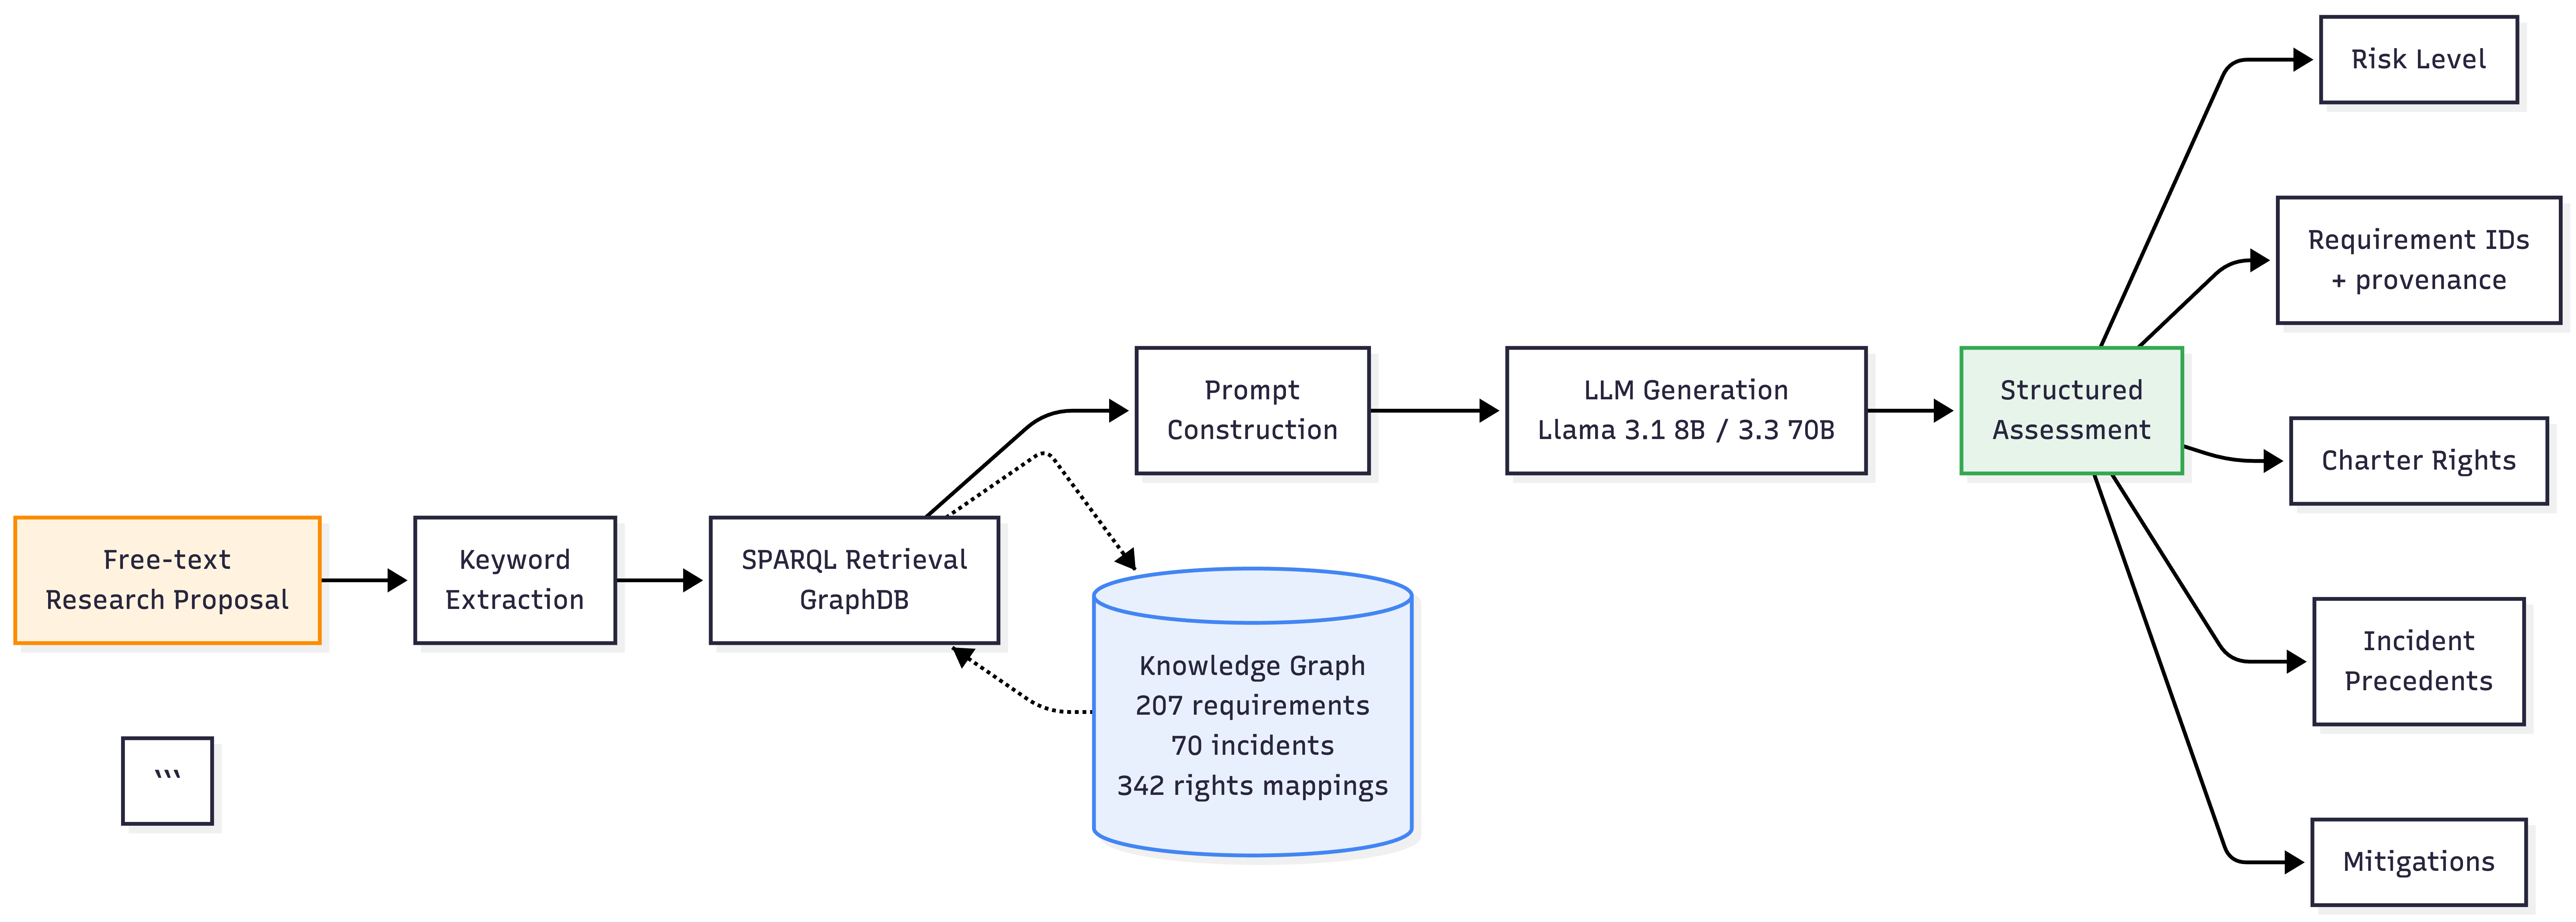
\includegraphics[width=0.95\textwidth]{architecture-flow.png}
\caption{AIEF system architecture: from free-text proposal to structured, traceable assessment.}
\label{fig:architecture}
\end{figure}

\section{Research Questions}

This paper is guided by three research questions. \textbf{RQ1:} Can a harmonised ontology effectively represent ethics assessment requirements across REAMS, the EU AI Act, Horizon Europe, and ACM/NeurIPS frameworks? \textbf{RQ2:} Can a knowledge graph populated with these requirements and real-world AI incidents support automated, rights-grounded ethics assessment? \textbf{RQ3:} Does retrieval-augmented generation over an ontology-driven knowledge graph produce more accurate and traceable assessments than an LLM operating without structured knowledge?

\section{Contributions}

This paper makes four contributions: (1) a harmonised ontology linking requirements from four governance frameworks to Charter articles, aligned with DPV and ODRL and published at \url{https://w3id.org/aief/}; (2) a knowledge graph of 207 requirements, 70 AI incidents, and 342 Charter rights mappings, validated through competency queries, an inter-annotator agreement study (Cohen's $\kappa = 0.712$), and the OOPS! pitfall scanner; (3) an empirically evaluated RAG assessment engine demonstrating 0.99 retrieval recall across model configurations and 90\% risk classification accuracy at the 70B scale, with an ablation isolating the knowledge graph's contribution; and (4) a deployed web application exposing the provenance of every cited requirement and incident.

%======================================================================
\chapter{Background and Related Work}
\label{ch:background}
%======================================================================

\section{The Cross-Framework Compliance Problem}

The four frameworks AIEF covers differ in scope and enforcement but overlap heavily in substance. REAMS v2 comprises 87 discrete requirements spanning consent, data protection, risk assessment, and institutional accountability \cite{reams2023}. The EU AI Act's Article 27 mandates Fundamental Rights Impact Assessments for high-risk systems \cite{euaiact2024}; AIEF encodes 30 FRIA-relevant requirements. Horizon Europe's Ethics by Design guidance specifies 52 requirements for funded research \cite{horizonethics2021}. The ACM Code and NeurIPS ethics guidelines contribute 38 \cite{acmethics2018, neurips2021}. Collectively these impose 207 requirements whose data-protection and risk-assessment obligations recur under different terminology and granularity. The EU Charter of Fundamental Rights, from which all four regimes ultimately derive legitimacy, provides a natural common reference: AIEF harmonises the frameworks by mapping each requirement to Charter articles, as illustrated in Figure~\ref{fig:kgschema}.

\begin{figure}[htbp]
\centering
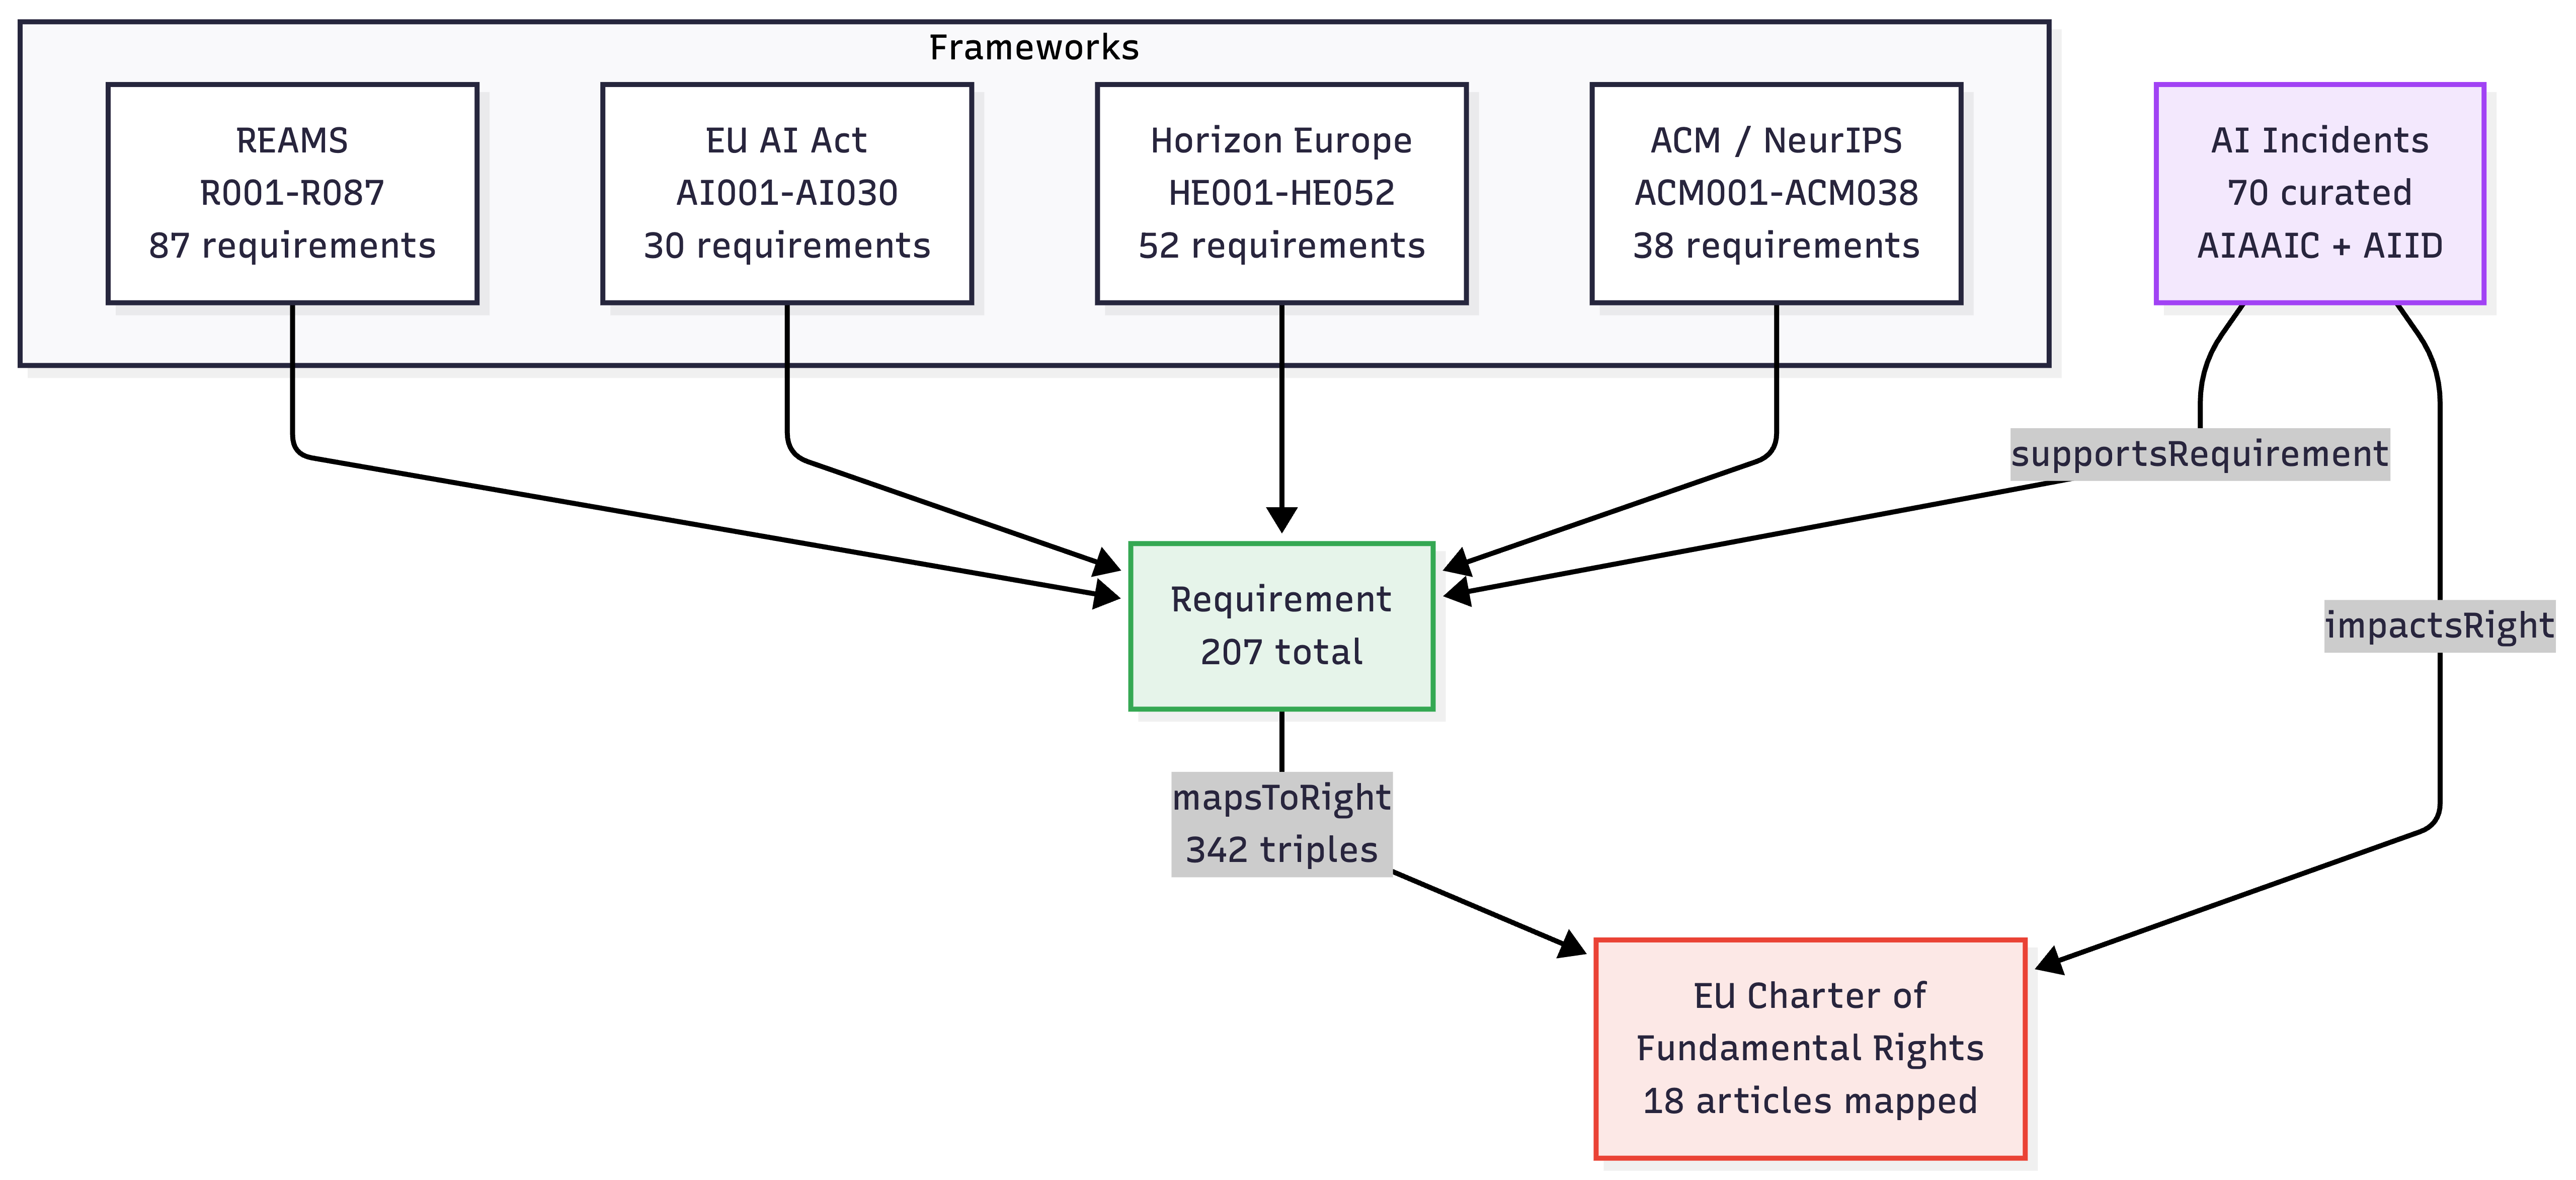
\includegraphics[width=0.9\textwidth]{kg-schema.png}
\caption{Knowledge graph schema: four governance frameworks harmonised through Charter rights mappings and grounded in curated AI incidents.}
\label{fig:kgschema}
\end{figure}

\section{Ontologies for AI Governance}

Pandit and Rintam\"{a}ki \cite{pandit2024fria} formalise FRIA as an OWL ontology extending the W3C Data Privacy Vocabulary (DPV) \cite{dpv2024}, and identify an automated assessment tool as future work. The AI Risk Ontology (AIRO) \cite{airo2022} provides a taxonomy of AI risks and harms aligned with the AI Act. The ITO knowledge graph \cite{ito2022} demonstrates large-scale incident knowledge engineering (1,100 classes) at a complexity exceeding the needs of a targeted compliance tool. AIEF draws on competency-question-driven design \cite{gruninger1995}, DPV alignment for rights interoperability, and ODRL \cite{odrl2018} for deontic modality.

\section{Retrieval-Augmented Generation for Compliance}

RAG grounds LLM generation in retrieved external knowledge \cite{lewis2020rag}. Gao et al.\ \cite{gao2023rag} establish the analytical separation of retrieval quality from generation quality that structures this paper's evaluation. RiskRAG \cite{riskrag2025} applies RAG to AI risk reporting from model cards but operates within a single framework, without an ontology, free-text input, or rights mapping. Farber \cite{farber2025} finds that LLM risk assessors systematically score risk higher than human assessors -- a conservative bias also observed here and discussed in Section~\ref{sec:risk-analysis}.

\section{Synthetic and Hybrid Evaluation}

Recent benchmarking work supports evaluating assessment systems on constructed scenarios complemented by real cases. PASTA \cite{pasta2026} evaluates AI outputs against multiple compliance policies simultaneously, validating system scores against a panel of human experts' median judgments -- a framework directly analogous to AIEF's multi-framework assessment and expert-review design. InvisibleBench \cite{invisiblebench2025} and AutoControl Arena \cite{autocontrolarena2025}, though situated in different AI-safety domains, demonstrate more broadly that researcher-constructed synthetic scenarios without real-participant data can support controlled, reproducible safety evaluation. Kapania et al.\ \cite{kapania2024} examine the ethics of using LLMs within HCI research practice, informing this paper's treatment of synthetic proposals as a substitute for confidential real REAMS applications.

\section{Participatory and Organisational Governance}

Two recent FAccT '26 contributions address AI governance from a complementary, organisational angle rather than an automated-tooling one. Jarvers and Papakyriakopoulos \cite{jarvers2026engaged} study the ``last mile'' problem of translating EU AI Act text into development practice, finding that practitioners perceive regulatory requirements inconsistently and arguing that internal expert collaboration, not automated tooling alone, is needed to close this gap. Ullstein et al.\ \cite{ullstein2026pafria} propose PaFRIA, a participatory Fundamental Rights Impact Assessment process developed iteratively with deployers, affected end-users, and experts.

Both papers reinforce a limitation AIEF shares with other automated assessment tools: neither internal-team buy-in nor affected-stakeholder participation is captured by a knowledge-graph-and-LLM pipeline operating on proposal text alone. AIEF and PaFRIA are complementary rather than competing: AIEF produces a rapid, traceable, pre-submission screen that could plausibly serve as an input artefact to a subsequent PaFRIA-style participatory process, surfacing candidate risks and rights for stakeholders to deliberate over rather than replacing that deliberation.

\section{Positioning}

To the best of our knowledge, no existing tool combines free-text proposal input, multi-framework coverage, a formal OWL ontology, an incident-grounded knowledge graph, Charter rights mapping, risk classification, and requirement-level traceability within a single pre-deployment assessment pipeline. Table~\ref{tab:comparison} summarises the comparison. AIEF's claim is integrative rather than component novelty: each ingredient exists in isolation; the contribution is their harmonisation into an operational, evaluated system that realises the tool prior work proposed.

\begin{table}[htbp]
\centering
\caption{Feature comparison with existing tools.}
\label{tab:comparison}
\small
\begin{tabular}{lccccc}
\toprule
\textbf{Feature} & \textbf{AIEF} & \textbf{ALTAI} & \textbf{RiskRAG} & \textbf{FRIA Ont.} & \textbf{AIRO} \\
\midrule
Free-text input        & \checkmark & --         & --         & --         & --     \\
Multi-framework        & \checkmark & --         & --         & --         & --     \\
OWL ontology            & \checkmark & --         & --         & \checkmark & \checkmark \\
KG with incidents       & \checkmark & --         & --         & --         & --     \\
Charter rights map      & \checkmark & Partial    & --         & \checkmark & --     \\
Risk classification     & \checkmark & \checkmark & \checkmark & --         & --     \\
Requirement IDs         & \checkmark & --         & --         & --         & --     \\
RAG pipeline             & \checkmark & --         & \checkmark & --         & --     \\
Pre-deployment scope    & \checkmark & --         & --         & \checkmark & --     \\
\bottomrule
\end{tabular}
\end{table}

%======================================================================
\chapter{System Design}
\label{ch:design}
%======================================================================

AIEF follows the Design Science Research paradigm \cite{hevner2004}: the artifact was constructed and evaluated over five design iterations (framework extraction, ontology design and expert review, knowledge graph population and validation, RAG pipeline construction, and evaluation).

\section{Ontology}

The ontology comprises 125 classes, 22 object properties, and 16 data properties, developed with competency questions and published at \url{https://w3id.org/aief/}. Six principal concepts organise the domain: \textsf{ResearchProposal}, \textsf{GovernanceRequirement} (subclassed per framework and by ODRL deontic modality), \textsf{FundamentalRight} (aligned with the DPV EU Fundamental Rights extension via \texttt{owl:equivalentClass}), \textsf{AIIncident}, \textsf{RiskLevel}, and \textsf{Mitigation}. Figure~\ref{fig:concept} illustrates the core class relationships. Key properties include \texttt{mapsToRight} (requirement $\to$ Charter article), \texttt{impactsRight} (incident $\to$ right), \texttt{supportsRequirement} (incident $\to$ requirement), and \texttt{demonstratesRisk}. The core \textsf{Requirement} and \textsf{Incident} individuals carry identifying data properties throughout; annotation coverage across the supporting-vocabulary classes is incomplete, as Section~\ref{sec:oops} reports.

\begin{figure}[htbp]
\centering

\includegraphics[width=0.85\textwidth]{concept-diagram.png}
\caption{AIEF ontology concept diagram: core classes and object properties.}
\label{fig:concept}
\end{figure}

The ontology was reviewed by a co-author of the FRIA ontology and AIRO; all seven review recommendations were implemented, including permanent namespace registration, DPV rights alignment, and ODRL subclassing.

\subsection{OOPS! Pitfall Scanner Validation}
\label{sec:oops}

The ontology was submitted in full to the OOPS! (OntOlogy Pitfall Scanner) web service \cite{poveda2014oops} on 14 July 2026, scanning against its standard 28-pitfall catalogue. The scanner returned 8 pitfall categories with at least one instance; none reached OOPS!'s highest (``Critical'') severity tier.

Two ``Important'' categories affect AIEF's own authored terms directly: \textbf{P11 (missing domain or range)} on 5 data properties (\texttt{incidentYear}, \texttt{coderAgreement}, \texttt{incidentTitle}, \texttt{incidentID}, \texttt{aiCapability}), and \textbf{P34 (untyped class)}, which affects mostly externally-referenced DPV rights terms (16 of 21 instances) rather than AIEF's own classes (2 of 21). A third Important category, \textbf{P10 (missing disjointness axioms)}, was flagged as a general recommendation with no specific elements enumerated. Five Minor categories were also reported, the most substantial being \textbf{P08 (missing annotations)} on 78 of AIEF's own elements -- chiefly supporting-vocabulary classes such as \textsf{PersonalData}, \textsf{DataSubject}, and \textsf{Researcher} -- and \textbf{P13 (inverse relationships not declared)} on 17 object properties. None of the eight findings indicate a structural or logical defect; all are annotation-completeness or property-declaration gaps addressable without redesigning the class hierarchy.

\section{Knowledge Graph}

\textbf{Requirements.} 207 requirements were manually extracted from source documents: REAMS R001--R087 (87), EU AI Act AI001--AI030 (30), Horizon Europe HE001--HE052 (52), ACM/NeurIPS ACM001--ACM038 (38). Each carries a unique identifier, source section reference, deontic modality, mandatory/tier classification, and Charter mappings; the 342 \texttt{mapsToRight} triples span 18 of the Charter's 54 articles. The populated graph contains 3,921 asserted triples, materialising to 4,847 under the RDFS+ ruleset used by the production GraphDB repository that the RAG pipeline queries at runtime (an earlier verification pass under a stricter OWL-Horst ruleset in a separate scratch repository reported 5,197; that figure did not reflect the ruleset actually used in production and has been superseded by this one).

\textbf{Incidents.} 70 incidents were curated from the AIAAIC Repository \cite{aiaaic2024} and the AI Incident Database \cite{aiid2024} across eight domain categories, selected by the researcher for representative coverage. Each incident is annotated with impacted rights, demonstrated risk categories, and the requirements it illustrates. A pilot inter-annotator study on ten incidents (540 binary decisions) yielded Cohen's $\kappa = 0.712$ -- substantial agreement \cite{landiskoch1977}.

\section{RAG Pipeline}

The pipeline comprises five modules: keyword extraction, SPARQL retrieval against GraphDB, prompt construction grounding the LLM in retrieved evidence, LLM generation (Ollama locally or Groq in the cloud), and structured output parsing into an eight-section assessment. Figure~\ref{fig:architecture} in Chapter~\ref{ch:introduction} shows the full pipeline; Figure~\ref{fig:ablation} in Chapter~\ref{ch:evaluation} shows how each stage contributes to the final assessment.

\section{Web Application}

A Next.js application deployed on Vercel (\url{https://aief.vercel.app}) provides public access. A retrieval-transparency panel juxtaposes the requirements retrieved from the knowledge graph with those the LLM cited, so users can verify that citations correspond to retrieved evidence.

%======================================================================
\chapter{Evaluation}
\label{ch:evaluation}
%======================================================================

\section{Design}

The dataset comprises 25 proposals: 20 synthetic proposals (P01--P20) stratified across risk levels (9 High, 7 Medium, 4 Low), and 5 documented real-world cases -- Optum \cite{optum2019}, COMPAS \cite{compas2016}, Amazon Rekognition \cite{rekognition2019}, Facebook ad delivery \cite{facebookads2019}, and the Epic Sepsis Model \cite{wong2021sepsis}. Four metrics were used: risk classification accuracy, retrieval recall, generation F1, and a three-condition ablation (LLM-only, KG-only, full pipeline), illustrated in Figure~\ref{fig:ablation}.

\begin{figure}[htbp]
\centering
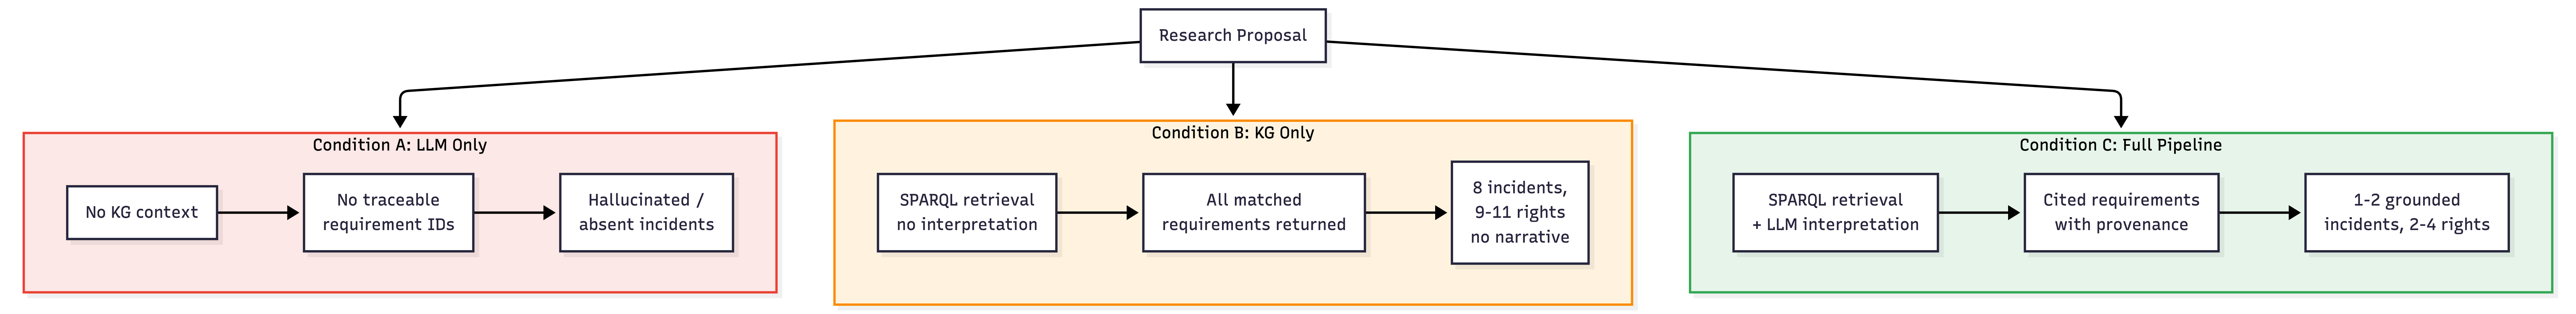
\includegraphics[width=0.95\textwidth]{ablation-methodology.png}
\caption{Ablation study design: isolating the knowledge graph's contribution from the LLM's.}
\label{fig:ablation}
\end{figure}

\section{Multi-Model Results}

\begin{table}[htbp]
\centering
\caption{Results by model configuration (20 synthetic proposals).}
\label{tab:results}
\begin{tabular}{lcc}
\toprule
\textbf{Metric} & \textbf{Llama 3.1 8B} & \textbf{Llama 3.3 70B} \\
\midrule
Risk classification accuracy & 65\% (13/20) & 90\% (18/20) \\
Retrieval recall & 0.99 & 0.99 \\
Generation F1 & 0.16 & 0.22 \\
Backend & Ollama (local) & Groq (cloud) \\
\bottomrule
\end{tabular}
\end{table}

Retrieval recall is 0.99 in both configurations, regardless of downstream model capacity, cleanly separating the knowledge engineering contribution from generation quality (Figure~\ref{fig:centralfinding}), following the retrieval/generation decomposition of Gao et al.\ \cite{gao2023rag}. This answers RQ1 and RQ2 affirmatively.

\begin{figure}[htbp]
\centering
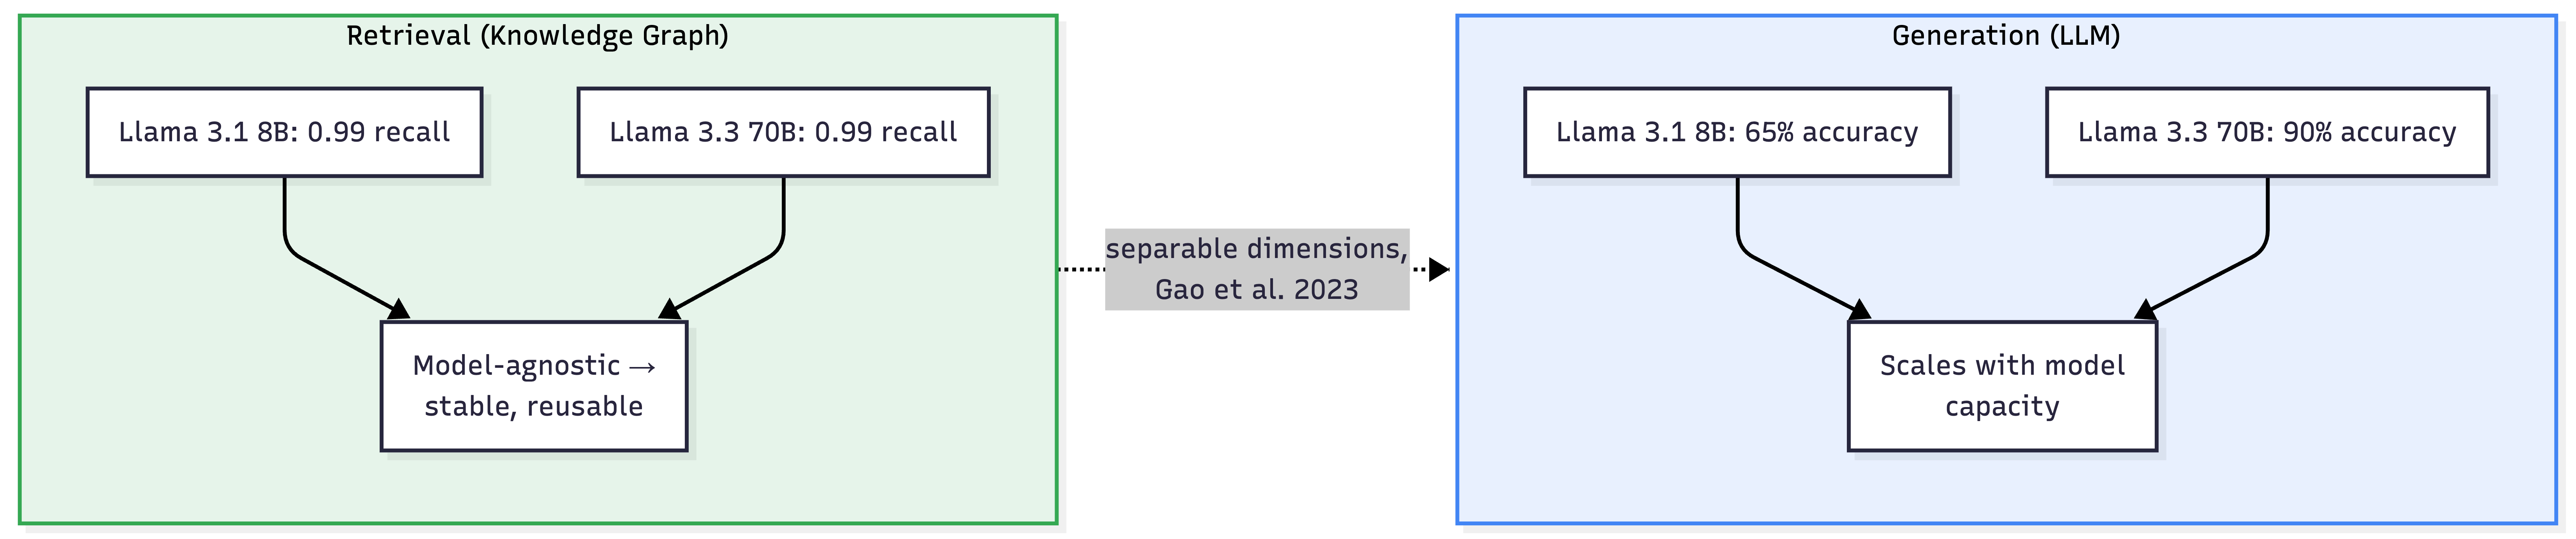
\includegraphics[width=0.9\textwidth]{central-finding.png}
\caption{Central finding: retrieval quality is model-agnostic; generation quality scales with model capacity.}
\label{fig:centralfinding}
\end{figure}

A third configuration (Qwen3 32B via Groq) is reported as exploratory only: 7 of 20 runs failed under free-tier tokens-per-minute rate limits, rendering comparison methodologically unreliable.
\label{sec:qwen-ratelimit}

\subsection{Risk Classification and Conservative Bias}
\label{sec:risk-analysis}

Accuracy scales with capacity (65\% $\to$ 90\%). The improvement from 65\% (13/20) to 90\% (18/20) reflects a 5-item difference on a 20-item sample and should be read as a directional trend consistent with the expected relationship between model capacity and reasoning accuracy, rather than a statistically established effect; no significance test was applied given the sample size, and a larger evaluation set is needed before the capacity-accuracy relationship can be treated as confirmed rather than suggestive. The 8B model's errors are systematically conservative: Medium and Low proposals are over-classified as High, while genuinely high-risk proposals are correctly flagged at 90\% even at 8B. In pre-deployment ethics screening this asymmetry is defensible -- a false negative is costlier than a false positive -- and aligns with the precautionary posture of EU AI Act Article 9. Farber \cite{farber2025} reports the same upward bias in LLM offender-risk assessment.

\section{Ablation}

Without the knowledge graph the LLM produces general ethics commentary with no traceable requirement identifiers and frequently fabricates incident precedents. The KG-only condition retrieves comprehensively but without interpretation. The full pipeline cites specific requirements with framework provenance, grounds its narrative in retrieved incidents, and synthesises a readable subset of the mapped rights -- directly answering RQ3.

\section{Real-World Cases}

Case descriptions were re-run through the deployed production system on 14 July 2026 rather than reported from memory, so the figures below are directly reproducible. All five documented cases were classified \textbf{High} risk, matching the documented severity of each case. Charter rights mappings closely tracked published analyses: Optum to Articles 21 and 35; COMPAS to Articles 21, 6, and 47; Rekognition to Articles 7, 8, and 21; Facebook ad delivery to Articles 21 and 23; and the Epic Sepsis Model to Article 21, citing requirements ACM003, HE013, and R085 and retrieving the Optum and Amazon hiring-bias incidents as precedents. The sample (n=5) still limits the strength of the external-validity claim.

\section{Automated RAG Metrics}

Four RAGAS-style metrics \cite{gao2023rag} were computed for all 20 synthetic proposals on 14 July 2026, then re-run on 15 July after a data-consistency issue was found and fixed in the production GraphDB repository (the corrected requirement graph existed on disk from 13 July but had not yet been reloaded into the live repository the RAG pipeline queries; context recall and precision were verified bit-for-bit identical before and after the fix, confirming the retrieval metrics were unaffected, while faithfulness and answer relevancy gained substantially fuller coverage on re-run). Context recall and precision (no LLM judge required) completed for all 20 proposals: mean recall 0.80 (range 0.00--1.00), mean precision 0.030 (range 0.006--0.065).

Precision should not be read as a tuned design parameter but as a consequence of keyword-based SPARQL retrieval being deliberately permissive: with 140--196 of 207 requirements typically surfaced per proposal, the retrieval stage functions closer to broad candidate filtering than to precise, targeted matching. This was an acceptable trade-off given the ethics-screening context, where a missed requirement (false negative) is more consequential than an irrelevant one being briefly surfaced (false positive). However, it also means the RAG pipeline's contribution is closer to ``near-complete context plus LLM triage'' than to precision-oriented retrieval, and the low precision should be read as a current limitation of the retrieval design rather than an intentionally optimised operating point.

Faithfulness and answer relevancy (Llama 3.3 70B as judge) completed for 19 of 20 proposals on re-run (one proposal, P20, retrieved zero context and was excluded from both judge metrics by construction): faithfulness averaged 0.35 (range 0.0--0.8), answer relevancy averaged 0.88 (range 0.5--1.0).

The faithfulness score (0.35) sits well below answer relevancy (0.88), a gap worth confronting directly rather than reporting in isolation. Three explanations are plausible and not mutually exclusive: first, the judge model (Llama 3.3 70B) is drawn from the same model family as the system under evaluation, which self-consistency literature suggests can bias faithfulness scoring in either direction depending on shared failure modes; second, retrieval surfaces 140--196 requirements per proposal (discussed above), and an LLM asked to synthesise a narrative from a near-complete requirement set may draw on background knowledge to fill gaps rather than citing only what was retrieved, which RAGAS-style faithfulness scoring penalises even when the output is substantively correct; third, faithfulness and answer relevancy are themselves LLM-judged scores and carry their own measurement uncertainty, evidenced by the fact that a full re-run on 15 July produced a materially different mean (0.35 versus 0.30 on 14 July's partial 5-proposal sample) despite querying an unchanged set of generated assessments. The high answer relevancy alongside low faithfulness suggests the pipeline produces on-topic, plausible assessments whose surface content is not always traceable to specific retrieved passages -- a distinction that matters for a tool whose central design goal is traceability, and one flagged as a priority for follow-up work rather than a settled negative result.

\section{Expert Review}

Scoring sheets covering eight proposals across five assessment dimensions (1--5 Likert) plus risk-level correctness were prepared for review by the supervisory team; inter-rater agreement and per-dimension medians will be reported once responses are received.

%======================================================================
\chapter{Discussion and Conclusion}
\label{ch:conclusion}
%======================================================================

\section{Threats to Validity and Limitations}

\textbf{Internal validity.} Synthetic-proposal ground truth was assigned by a single researcher. \textbf{External validity.} Real institutional ethics applications are confidential; five real-world cases mitigate but do not remove this gap. \textbf{Construct validity.} The Medium/High risk boundary is contextually debatable. \textbf{Reliability.} LLM outputs are stochastic; results reflect single runs at fixed temperature. Given that risk classification accuracy is the paper's central quantitative claim, repeated runs per proposal (to characterise output variance) and a second independent annotator for ground-truth labelling are identified as immediate priorities for strengthening this result, rather than generic future work.

Further limitations: coverage is four frameworks; the 70-incident corpus requires periodic refresh; keyword-based SPARQL retrieval may miss requirements phrased differently from the proposal; and retrieval precision is low by design (Chapter~\ref{ch:evaluation}).

\section{Conclusion}

AIEF demonstrates that an ontology-driven knowledge graph combined with retrieval-augmented generation can deliver automated, traceable, rights-grounded ethics assessments of free-text AI research proposals across four governance frameworks simultaneously. The evaluation's central result -- 0.99 retrieval recall invariant across model scale, with risk accuracy rising from 65\% to 90\% with model capacity -- establishes that the knowledge engineering layer is a stable, reusable asset whose value is independent of the LLM that consumes it. Future work includes framework extension, semi-automated incident ingestion, hybrid embedding retrieval, remediating the OOPS!-identified pitfalls, improving retrieval precision, completing the expert-review study, and investigating how AIEF's automated screen could feed into a participatory review process involving affected stakeholders \cite{jarvers2026engaged,ullstein2026pafria}. The ontology, knowledge graph, pipeline, evaluation outputs, and web application are publicly available at \url{https://w3id.org/aief/} and \url{https://github.com/navinaamuthan/ai-ethics-framework-tool}.

\bibliographystyle{plain}
\bibliography{bibs/references}

\end{document}
